
\documentclass[12pt,oneside]{book}
\usepackage{graphicx}

% enable onehalfspaceing etc
\usepackage{setspace}

% Make chapter enumeration big and fat
\usepackage{fix-cm}
\usepackage{xcolor}
\usepackage[bf,rm,medium,compact]{titlesec}
\definecolor{gray75}{gray}{0.75}
\newcommand{\hsp}{\hspace{20pt}}
\titleformat{\chapter}[display]{\filleft\Huge\bfseries}{\fontsize{100}{100}\selectfont\textcolor{gray75}\thechapter}{1ex}{}[]%


% Enable non-ugly hyperlinks
\usepackage{blindtext}
\usepackage[hidelinks]{hyperref}


% =============Manually Added Packages======================
% Add image in the cover page at the bottom right corner
\usepackage{tikz}
% =============Manually Added Packages======================


% Some metadata for your generated PDF
\title{Masters Thesis}
\author{Prasannjeet Singh}
\date{\today}

% DOCUMENT BEGINS
\begin{document}


% Special command to link to official guidelines:
\newcommand{\mcgillguidelines}{\href{https://www.mcgill.ca/gps/thesis/thesis-guidelines/preparation}{Official McGill Guidelines: }}


% TITLE PAGE
\begin{onehalfspacing}
\pagestyle{empty}
% This title page conforms to the mcgill university wide thesis guidelines:
% https://www.mcgill.ca/gps/thesis/thesis-guidelines/preparation

% Students can request permission to add the official McGill logo to their thesis cover page by submitting this webform: https://www.mcgill.ca/visual-identity/application-use-university-logo-demande-dutilisation-du-logo-de-luniversite


\begin{titlepage}
\begin{center}

\vspace*{0.5cm}


{\bfseries\LARGE  AiMentalAcoustics}
\vspace{0.15cm}

{\bfseries\LARGE  Contactless AI-assistive system to}
\vspace{0.15cm}

{\bfseries\LARGE  recognize, detect, and forecast for mental wellness}
\vspace{1.8cm}

{\large Prasannjeet Singh}
% \\Doctor of Philosophy

% Institution
\vspace{1cm}
% The McGill Logo
% NOTE: YOU HAVE TO ASK FOR PERMISSION TO INTEGRATE THE LOGO. YOU CAN GET IT HERE: https://www.mcgill.ca/visual-identity/application-use-university-logo-demande-dutilisation-du-logo-de-luniversite
\begin{figure}[ht!]
    \centering
    
\includegraphics[width=.8\linewidth]{images/Lnu_Wordmark_Symbol_Sweden_Eng_rgb.png}
  \end{figure}
Department of Computer Science and Media Technology\\
Linnaeus University\\
Växjö, Sweden\\

\vspace{1.5cm}
\today


% More prosa about the university falala mcgill is so great.
\vspace{1.0cm}
\noindent
A thesis submitted to Linnaeus University in partial\\
fulfillment of the requirements of the degree of\\
Masters in Software Technology

% Add a copyright for your name, just in case.
\vspace{1.0cm}
{\small \copyright Prasannjeet Singh, \the\year{}}


\end{center}

\begin{tikzpicture}[remember picture,overlay]

    \node[anchor=south east, inner sep=0pt, xshift=-1cm, yshift=1cm] at (current page.south east) {
\includegraphics[width=2cm]{images/Lnu-se_rgb.png}};

    \node[anchor=south west, inner sep=0pt, xshift=-3cm, yshift=-1cm] at (current page.south west) {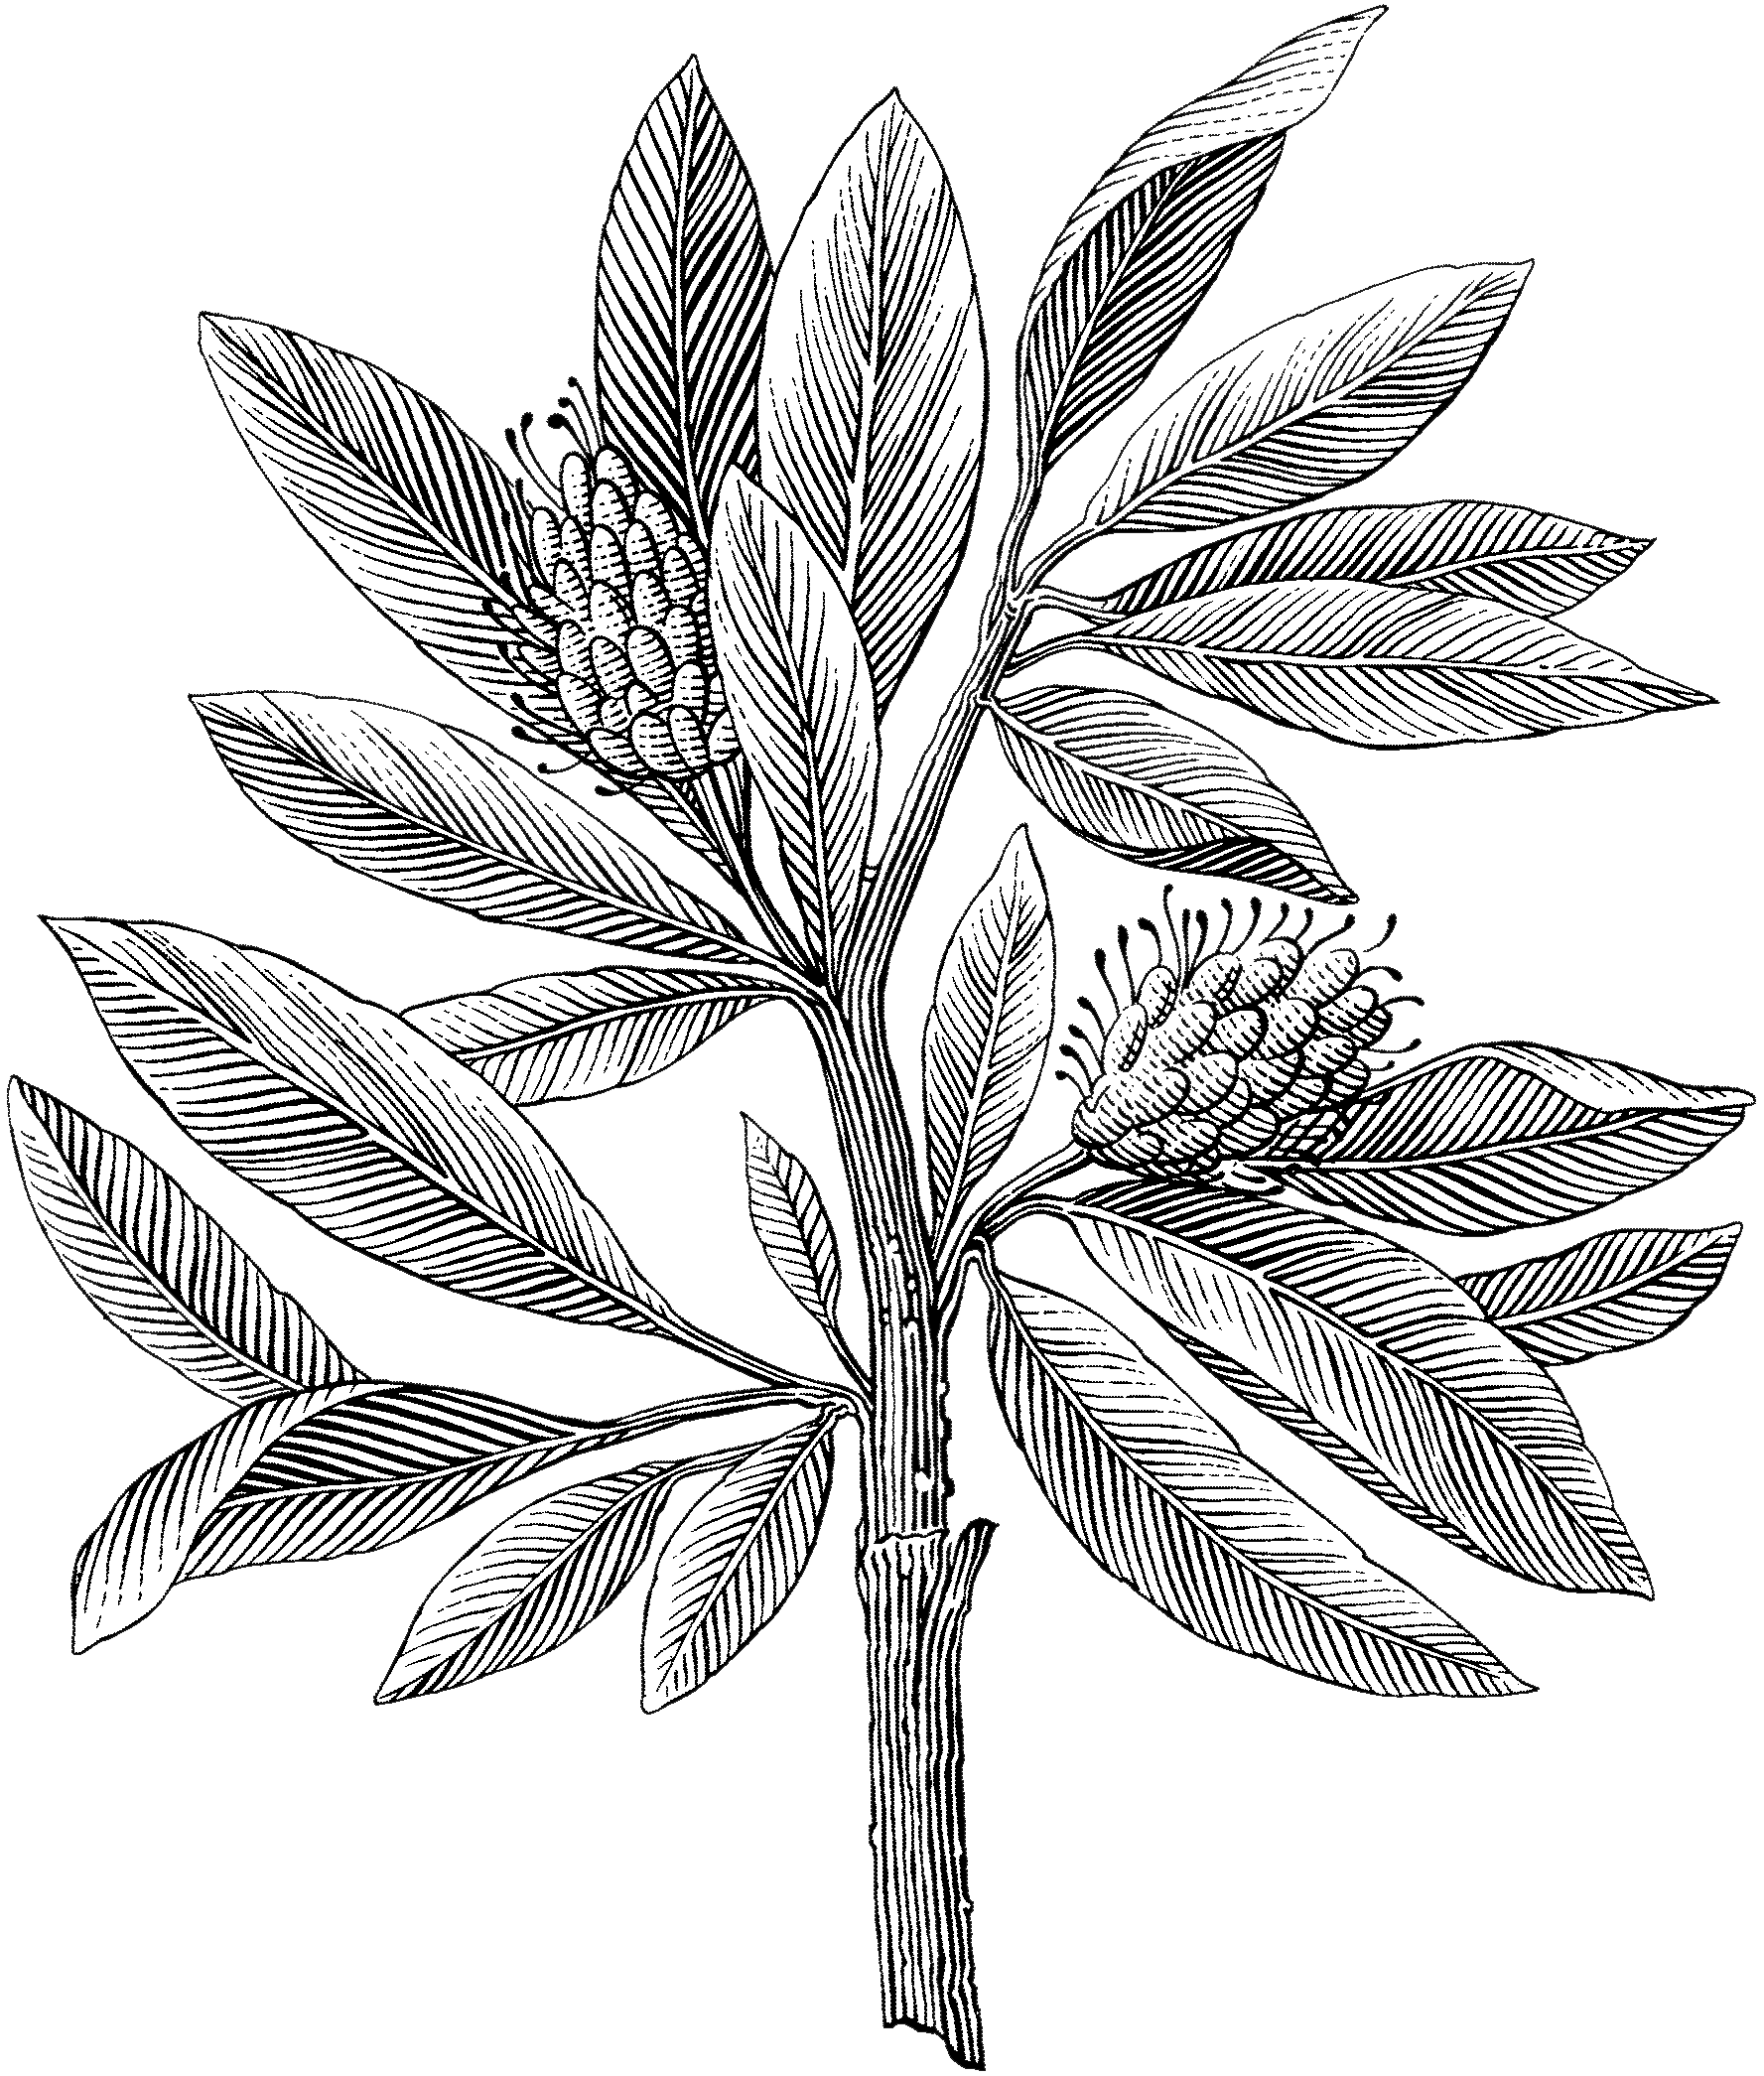
\includegraphics[width=10cm]{images/lnu_copperplate_inv.png}};

    \node[anchor=north west, inner sep=0pt, xshift=1cm, yshift=-1cm] at (current page.north west) {
\includegraphics[width=2.5cm]{images/logo_yellow.jpg}};
\end{tikzpicture}


\end{titlepage}






\cleardoublepage
\end{onehalfspacing}


% Pages in all "Chapters" before the actual thesis content are enumerated in roman (i, ii, iii, ...)
\pagenumbering{roman}
\pagestyle{plain}


% Abstracts in English and French
\chapter*{\rm\bfseries Abstract}
\label{ch:abstraten}

\href{https://www.mcgill.ca/gps/thesis/thesis-guidelines/preparation}{Official McGill Guidelines}: If the language of the thesis is neither English nor French (only allowed for specific language Units) then a third abstract in the language of the thesis is required.

Abstracts in English and French are mandatory and must be text only, i.e. no images, special characters (apart from the West European character set excluding the “Œ” and “œ”), chemical or mathematical formulae, or special formatting (e.g. lists, tables). Abstracts have a maximum limit of 4000 characters.
\clearpage
% \chapter*{\rm\bfseries Abr\'eg\'e}
\label{ch:abstratfr}

\href{https://www.mcgill.ca/gps/thesis/thesis-guidelines/preparation}{Official McGill Guidelines}: La même chose en français.
\cleardoublepage


% List of Contributions
% Abstracts in English and French
\chapter*{\rm\bfseries Contribution}
\label{ch:contribution}

\href{https://www.mcgill.ca/gps/thesis/thesis-guidelines/preparation}{Official McGill Guidelines}: A doctoral thesis must clearly state the elements of the thesis that are considered original scholarship and distinct contributions to knowledge.

\begin{itemize}
    \item{Contributions of the student to each chapter must be explicitly stated.}
    \item{Contributions of any co-authors to each chapter must be explicitly stated.}
\end{itemize}


 
\clearpage


% Acknowledgements
\chapter*{\rm\bfseries Acknowledgements}
\label{ch:acknowledgement}

\href{https://www.mcgill.ca/gps/thesis/thesis-guidelines/preparation}{Official McGill Guidelines}: Among other acknowledgements, the student is required to declare the extent to which assistance (paid or unpaid) has been given by members of staff, fellow students, research assistants, technicians, or others in the collection of materials and data, the design and construction of apparatus, the performance of experiments, the analysis of data, and the preparation of the thesis (including editorial help).


\begin{itemize}
    \item{In addition, it is appropriate to recognize the supervision and advice given by the thesis supervisor(s) and advisors.}
\end{itemize}
\clearpage

% Next comes the GENERATED list of contents, figures and tables.
\tableofcontents
\listoffigures
\listoftables
\clearpage

% Here comes the actual thesis content, we switch back to arabic page numbers.
\pagenumbering{arabic}
% \pagestyle{fancyplain}


\chapter{\rm\bfseries Introduction}
\label{ch:chapter01}

\section{Background}

\begin{itemize}
\item{Brief on the importance of EEG in cognitive studies.}
\item {The significance of the research in the current scientific landscape.}
\end{itemize}

\section{Aim and Objectives}

\begin{itemize}
\item{Clear statement of the research aim.}
\item{Specific objectives to be achieved.}
\end{itemize}
\chapter{\rm\bfseries Literature Review}
\label{ch:chapter02}

\section{Historical Context}
\begin{itemize}
    \item Evolution of EEG studies.
\end{itemize}

\section{Previous Works}
\begin{itemize}
    \item Summarize key studies in the domain.
\end{itemize}

\section{Gaps in Existing Literature}
\begin{itemize}
    \item Identify areas that haven't been explored or need further investigation.
\end{itemize}
\chapter{\rm\bfseries Ethical Considerations}
\label{ch:chapter03}

\section{Importance of Ethics in EEG Studies}

\section{Ethical Approval Process}
\begin{itemize}
    \item Detailed description of the process of obtaining ethical approval from the Swedish Ethical Review Authority (Etikprövningsmyndigheten).
    \item Importance of ensuring participant anonymity and data privacy.
\end{itemize}

\section{Participant Consent}
\begin{itemize}
    \item Process of informing participants.
    \item Ensuring voluntary participation and the right to withdraw.
\end{itemize}


\chapter{\rm\bfseries Methodology}
\label{ch:conclusions}

\section{Participant Selection}
\begin{itemize}
    \item Criteria for selection and exclusion.
\end{itemize}

\section{EEG Test Procedure}
\begin{itemize}
    \item Detailed steps of how the test is conducted.
\end{itemize}

\section{Data Collection and Analysis}
\begin{itemize}
    \item Tools and techniques used for data collection.
    \item Methods for analyzing the collected data.
\end{itemize}




\chapter{\rm\bfseries Technical Implementation}
\label{ch:techimpl}

\section{Quiz Architecture}
\begin{itemize}
    \item Overview of the quiz system.
    \item Role of AngularJS in the frontend.
\end{itemize}

\section{EEG Data Recording System}
\begin{itemize}
    \item Integration of the Python service for EEG data recording.
    \item Automation of the recording process.
\end{itemize}

\section{Backend and Data Storage}
\begin{itemize}
    \item Role of the Spring backend in data storage.
    \item Ensuring data privacy and security using Key Cloak.
\end{itemize}

\chapter{\rm\bfseries Results and Discussion}
\label{ch:results_and_discussion}

\section{Data Presentation}
\begin{itemize}
    \item Graphs, tables, and other visual representations of the collected data.
\end{itemize}

\section{Interpretation}
\begin{itemize}
    \item Analysis of the results in the context of the research objectives.
\end{itemize}



\chapter{\rm\bfseries Conclusion}
\label{ch:conclusion}

\section{Summary of Findings}

\section{Implications for Future Research}
\begin{itemize}
    \item How this research can pave the way for future studies.
\end{itemize}

\section{Limitations}
\begin{itemize}
    \item Any constraints or limitations encountered during the research.
\end{itemize}




% List of YOUR publications
\chapter*{\rm\bfseries Publications}
\label{ch:publications}

This part is optional, but it gives a nice touch to list all the publications (official venues down to poster sessions) throughout your PhD.

Keep this in the same style as publications in your academic CV: 
Conference / Year - Title - Authors. And here comes a sample ref for the bibliography: \cite{schiedermeier_fiddlr_2021} and \cite{schiedermeier_fiddlr_2021} and finally \cite{schiedermeier_fiddlr_2021}.



% Optional: List of Acronyms / Glossary
\chapter*{\rm\bfseries Acronyms}
\label{ch:acronyms}

This part is likewise optional. But it does not hurt to provide a list of all acronyms, e.g.:

\begin{itemize}
    \item{\textbf{REST}: \textbf{Re}presentational \textbf{S}tate \textbf{T}ransfer}
\end{itemize}


% Finally your references
% PLEASE use a management system, e.g. Zotero (this works really nice with overleaf, there's seamless referencing of all your organized papers from zotero).
% To add zotero, use "New file -> From Zotero"
\bibliographystyle{alpha}
\bibliography{references}

\end{document}